\documentclass[a4paper,12pt]{report}

\usepackage{alltt, fancyvrb}
\usepackage{xurl}
\usepackage{graphicx}
\usepackage{xcolor}
\usepackage[utf8]{inputenc}
\usepackage{float}
\usepackage{hyperref}
\usepackage[italian]{babel}
\usepackage[italian]{cleveref}

\title{\textbf{Relazione per\\``Yokimon''}}
\author{Federico De Leonardis\\Luca Palazzini\\Marilia Merendi\\Giovanni Paone}
\date{25 Febbraio 2024}
\begin{document}
\maketitle
\tableofcontents
\chapter{Analisi}
\section{Requisiti}
Il software mira alla creazione di un videogame ispirato ai classici titoli di Pokémon, completo di mappa da esplorare, creature da catturare e nemici da sconfiggere tramite combattimenti a turni. A differenza della saga originale, Yokimon presenta una versione roguelike del gameplay. 
%
Con roguelike si intende un genere di videogame nel quale i livelli (o, come in questo caso, la mappa da esplorare) sono generati proceduralmente e pertanto diversi ad ogni run, e che non permette di preservare i propri progressi anche dopo una sconfitta. 
%
Il player, così come i suoi avversari, potrà disporre di più Yokimon da utilizzare in combattimento.
\subsubsection{Requisiti funzionali}
\begin{itemize}
    \item \textbf{Mappa} \\
    La mappa verrà generata proceduralmente ad ogni partita. 
    %
    Essa è composta da \texttt{Tile}, ovvero schermate di gioco, che avranno delle direzioni connesse specifiche e contenenti varie entità, ad esempio altari e nemici. 
    %
    Il player potrà muoversi per il \texttt{Tile} liberamente, e per la mappa in qualsiasi direzione (se il tile stesso lo permette), ed interagire con i nemici (\texttt{Enemy}) per iniziare combattimenti o con gli altari per ottenere nuovi Yokimon. Una volta sconfitte tutte le entità enemy sulla mappa, la partita si potrà definire conclusa.
    \item \textbf{Yokimon} \\
    Yokimon, figure ispirate agli yokai del folklore giapponese, sono spiriti in grado di combattere che possono essere sia ai comandi del player che a quelli dei nemici.
    %
    Sono caratterizzati da statistiche di base intrinseche determinate dal tipo di spirito (base stats), dalle quali derivano le statistiche effettive (stats) proprie di ogni livello, le uniche che effettivamente verranno considerate durante il combattimento. 
    %
    Esse determinano la forza, la difesa, la velocità e i punti vita di uno Yokimon e possono migliorare a seguito di un level-up. Infine gli Yokimon, così come i loro attacchi, sono caratterizzati da dei colori, che definiscono le affinità durante il combattimento: \\
    %
    \color{red}RED\color{black}: resistenti contro \textbf{BLACK} e deboli contro \color{violet}PURPLE\color{black}\hspace{1pt} e \color{red}RED\color{black} \\
    %
    \textbf{BLACK}: resistenti contro \color{violet}PURPLE\color{black}\hspace{1pt} e deboli contro \color{red}RED\color{black}\hspace{1pt} e \textbf{BLACK} \\
    %
    \color{violet}PURPLE\color{black}: resistenti contro \color{red}RED\color{black}\hspace{1pt} e deboli contro \textbf{BLACK} e \color{violet}PURPLE\color{black} \\
    %
    WHITE: colore neutro, nessuna affinità particolare con gli altri tipi. \\
    %
    Tutti i colori, tranne WHITE, fanno meno danno contro gli Yokimon della stessa tipologia.
    \item \textbf{Combattimento} \\
    Il combattimento si svolgerà a turni.
    %
    Il player e il suo avversario si alterneranno negli attacchi, fino a che uno dei due non resterà senza più Yokimon da poter usare in combattimento. In particolare, uno Yokimon non è più utilizzabile quando esaurisce i suoi HP points (healing points, “punti vita”).
    %
    In caso di vittoria del player, lo Yokimon che sta attualmente utilizzando riceverà degli XP points (experience points, “punti esperienza”) che potrà usare per fare level-up e incrementare le sue stats.
\end{itemize}
\subsubsection{Requisiti non funzionali}
L’applicazione non presenta particolari requisiti relativi ad efficienza, performance o sicurezza.
\section{Analisi e modello del dominio}
Il player sarà rappresentato da un \texttt{Entity} specifica (\texttt{Player}).
%
Il gioco si svolge in due settings distinti, quello della mappa da esplorare e quello del combattimento.
%
Nel primo, il player si muove nella mappa (\texttt{GameMap}), composta da unità dette \texttt{Tiles}. Il player può esplorare liberamente la mappa e qui vi può trovare degli altari (\texttt{Altar}), nei quali può ricevere degli \texttt{Yokimon}, e degli \texttt{Enemy}, che lo seguiranno per iniziare il combattimento.
%
Durante il combattimento (\texttt{Fight}), il \texttt{Player} e l’\texttt{Enemy} mettono in campo uno \texttt{Yokimon} per volta (il combattimento è esclusivamente 1 vs 1) e si sfidano tramite mosse (\texttt{Attack}).
%
Se il \texttt{Player} vince, il suo ultimo \texttt{Yokimon} coinvolto nel combattimento riceve degli XP Points, grazie ai quali può fare level-up. 
%
Se il \texttt{Player} perde, è game over.
%
Gli elementi costitutivi del problema sono sintetizzati in \Cref{img:uml-main}.
\begin{figure}[H]
\centering{}
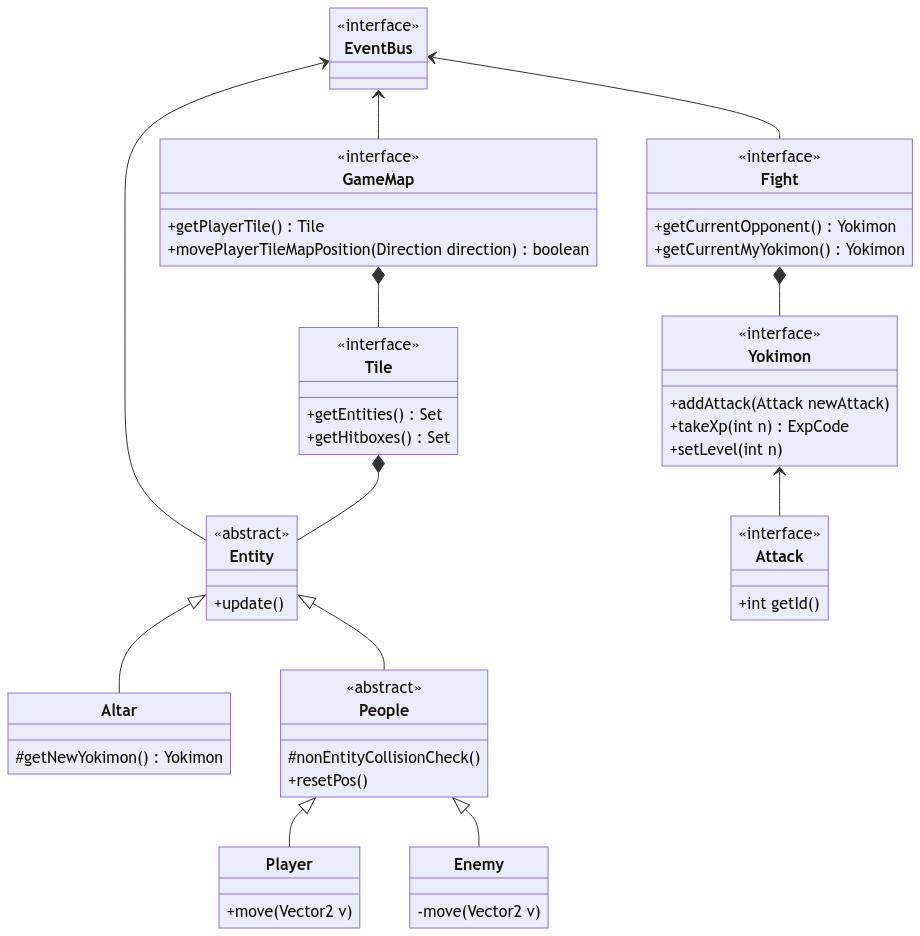
\includegraphics[width=1.0\columnwidth]{images/uml-1-2.png}
\caption{Schema UML dell’analisi del problema, con rappresentate le entità principali ed i rapporti fra loro}
\label{img:uml-main}
\end{figure}
\chapter{Design}
\section{Architettura}
Yokimon segue il pattern MVC non come visto a lezione, ma nella forma in cui è stato concepito da Trygve Reenskaug\footnote{\href{https://youtu.be/o_TH-Y78tt4?si=lk4vbCll47vFUt1A&t=1659}{The Principles of Clean Architecture by Uncle Bob Martin}}. 
%
In questa versione, il Controller agisce sul Model e il Model agisce sulla View tramite il sistema di observer. 
%
Controller e View pertanto non presentano dipendenze dirette.
\\
\begin{figure}[H]
\centering{}
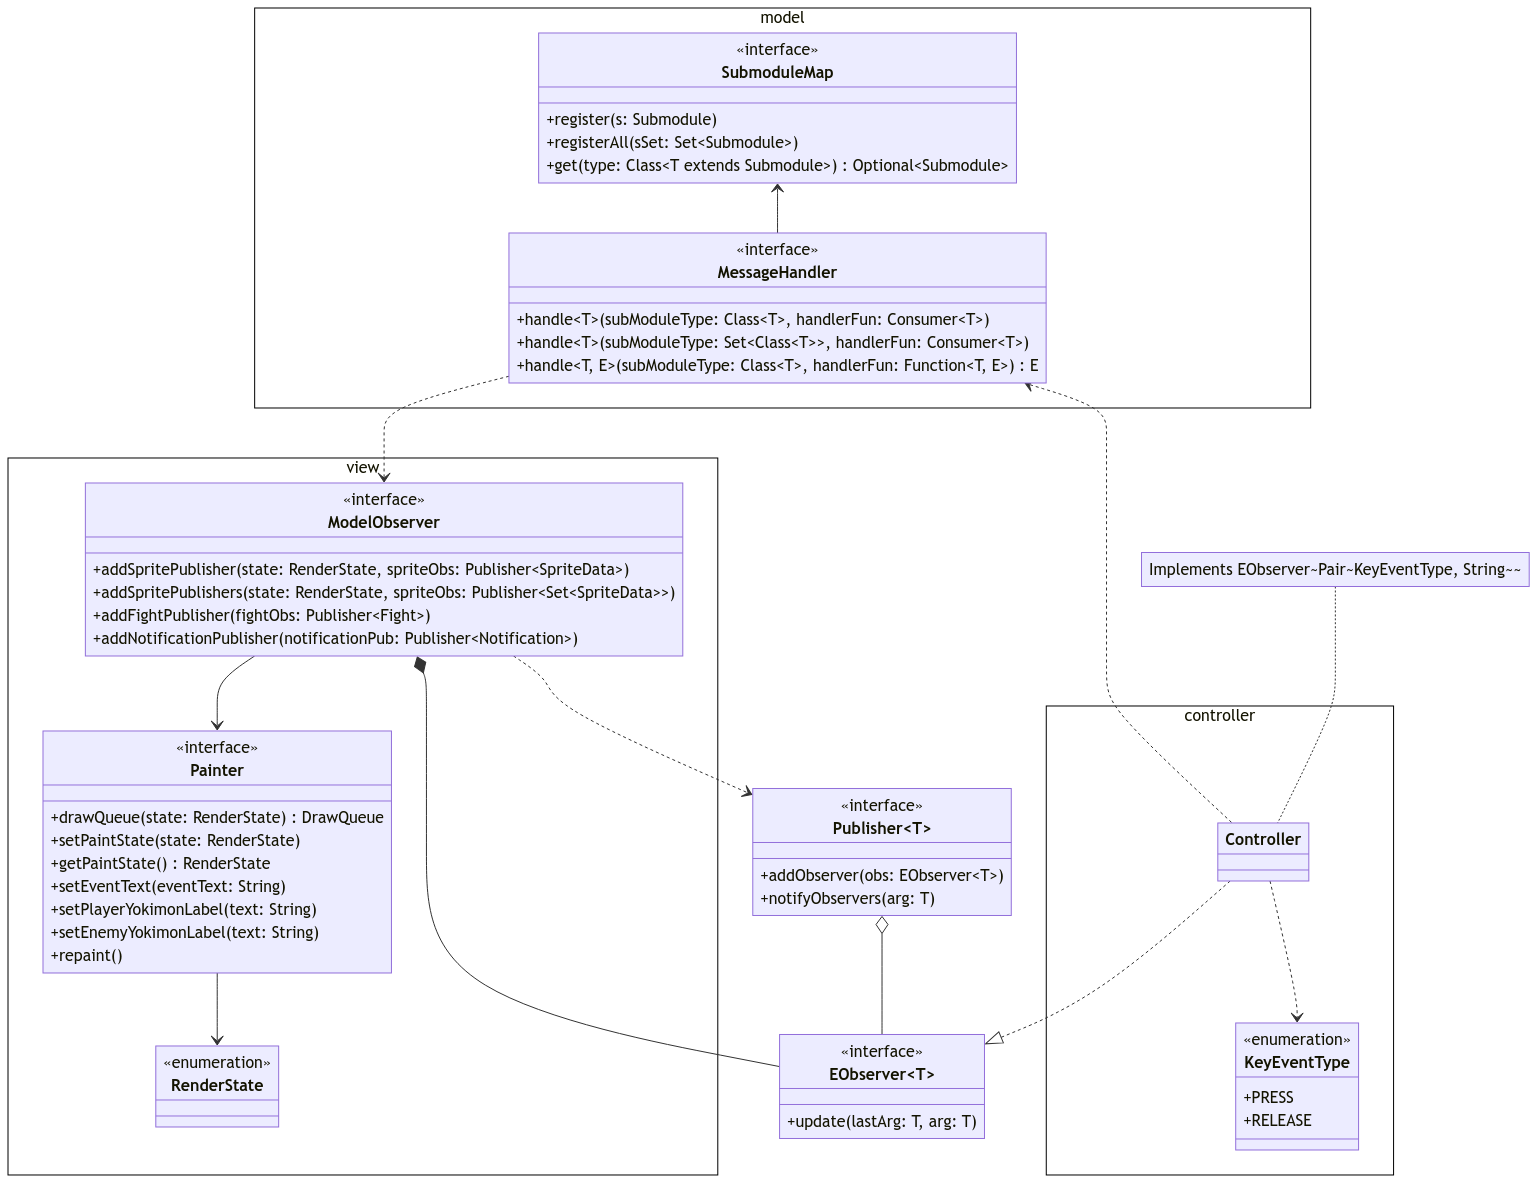
\includegraphics[width=1.0\columnwidth]{images/uml-mvc.png}
\caption{Schema UML che descrive il nostro utilizzo dell'MVC pattern}
\label{img:uml-mvc}
\end{figure}
Il \texttt{MessageHandler} è il bus centrale che rappresenta il modello, contiene una selezione di sottomoduli e fornisce un sistema di comunicazione per essi, dando l’opportunità al Controller di segnalare eventi di input che riceve dai publisher a cui è iscritto.
%
Il \texttt{MessageHandler} viene inizializzato con un ModelObserver che viene usato per collegare mediante Publisher i vari eventi di interesse della view alla rappresentazione di stato che possiedono i vari sottomoduli.
%
Da notare che sia Controller che \texttt{ModelObserver} presentano solamente una relazione di dipendenza nei confronti di \texttt{MessageHandler}, essi vengono solamente coinvolti nell’inizializzazione: Nel caso del \texttt{Controller} esso estrae le chiamate necessarie per comunicare al modello il cambio di stato in Consumer, il \texttt{ModelObserver} invece viene passato nell’inizializzazione del \texttt{MessageHandler} e di tutti i sottomoduli che contiene per associare gli observer forniti dalla view ai publisher contenuti nei sottomoduli. \\
%
Il bus di comunicazione che fornisce il \texttt{MessageHandler} è tratto dal design pattern del Command. \\
%
\texttt{GameWindow} rappresenta l’istanziatore della finestra di gioco. \\
%
\texttt{Painter} si occupa di rappresentare a schermo i dati che vengono ricevuti dagli observer di \texttt{ModelObserver}. 
%
Una implementazione di painter sarà quindi dipendente dalla libreria che istanzierà e gestirà la finestra.
\section{Design dettagliato}
\subsubsection{De Leonardis Federico}
\subsubsection{Entity-system}
\begin{figure}[H]
\centering{}
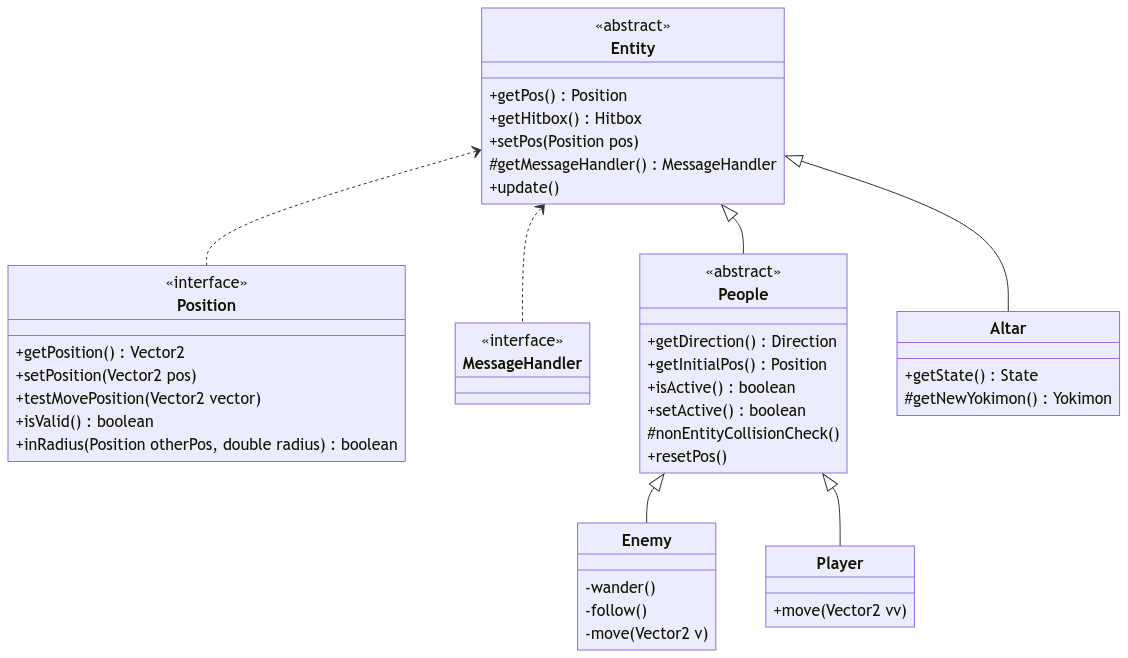
\includegraphics[width=1.0\columnwidth]{images/uml-entity.png}
\caption{Schema UML che descrive la classe \texttt{Entity} e le sue componenti}
\label{img:uml-entity}
\end{figure}
\paragraph{Problema} La sfida principale di questa parte consiste nel creare una serie di classi che definiscono come oggetti le varie \texttt{Entity} presenti nella mappa di gioco, dall’altra gli \texttt{Yokimon} presenti nel sistema di combattimento. 
%
Per quanto riguarda la prima parte, dato che sono presenti 3 tipologie di entità nella logica mappa di gioco, cioè \texttt{Enemy} (i nemici), \texttt{Altar} (gli altari) e \texttt{Player} (il personaggio controllato dall’utente), è facile notare come esse abbiano varie caratteristiche in comune.
\paragraph{Soluzione} Perciò ho utilizzato il design pattern template method per evitare il più possibile casi di codice e funzionalità duplicate, creando una classe astratta Entity, contenente sia metodi sia campi comuni a tutte le successive implementazioni, più il metodo astratto \texttt{update()}. 
%
Quest’ultima scelta è data dal fatto che in questo modo sarà possibile chiamare durante il game loop questo metodo per ciascuna delle entità senza per forza sapere il tipo e senza passare in input parametri diversi. Essa dipende da un’interfaccia \texttt{Position}, che semplifica la gestione delle posizioni, e da un \texttt{MessageHandler}, che permette lo scambio di informazioni e parametri senza bisogno del loro passaggio in possibili campi o parametri di metodi. 
%
\texttt{Entity} viene quindi implementata da \texttt{Altar} ed espansa da \texttt{People}, un'altra classe astratta che contiene metodi e funzionalità comuni sia a \texttt{Enemy}, sia a \texttt{Player}, come il controllo delle collisioni o la direzione in cui è rivolta l’entità. 
%
\texttt{Enemy} e \texttt{Player} implementano quindi in modo separato la gestione del movimento delle stesse a seguito di un update. 
%
Sono rispettati i principi SRP e OCP, dato che potenzialmente con questo modello possono essere aggiunte nuove entità facilmente, come ad esempio un Boss (effettivamente una classe estesa da enemy) o un Mercante. 
%
Si è inoltre deciso di evitare l’uso di interfacce per questo problema, dal momento che le entità istanziabili implementano già delle classi astratte. Ci è sembrato opportuno non aggiungere complessità eccessiva al model.
\subsubsection{Yokimon-system}
\begin{figure}[H]
\centering{}
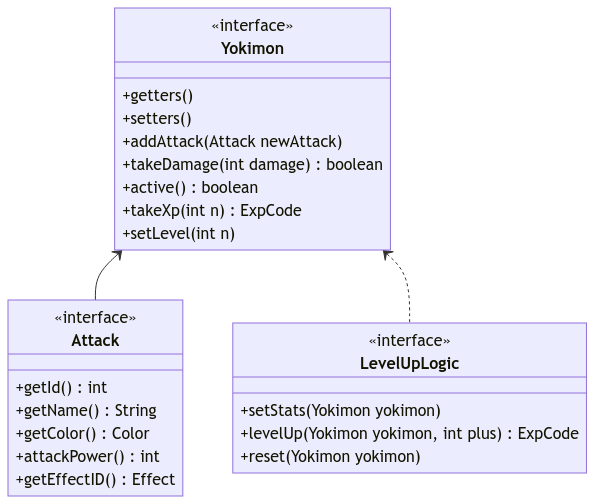
\includegraphics[width=1.0\columnwidth]{images/uml-yokimon.png}
\caption{Schema UML della interfaccia \texttt{Yokimon}}
\label{img:uml-yokimon}
\end{figure}
\paragraph{Problema} Il problema di questa parte stava nel modellizzare degli \texttt{Yokimon} con varie statistiche e relativi attacchi, utilizzabili in combattimento e ottenibili dal player tramite altari. 
%
Devono inoltre essere facilmente maneggevoli da altre classi che si occupano del combattimento o del caricamento da file da parte dei loader.
\paragraph{Soluzione} Anche in questo caso vengono rispettati i principi DIP, OCP e SRP in quanto \texttt{Yokimon} è definita come un’interfaccia con la sua relativa implementazione, che risponde all’esigenza di dipendere da interfacce. 
%
I metodi sono dichiarati finali, in quanto si desidera che la classe non venga modificata, ma potenzialmente in futuro estesa.
%
La maggior parte della logica è scorporata dalla classe principale, che dipende dall’interfaccia \texttt{LevelUpLogic}, la cui implementazione permette di gestire in modo pratico la relativamente complessa meccanica di level-up degli \texttt{Yokimon} e la possibilità di ri-settare il livello di uno \texttt{Yokimon} o di acquisire punti esperienza con una sola chiamata di metodo.
\subsubsection{Generation factory}
\begin{figure}[H]
\centering{}
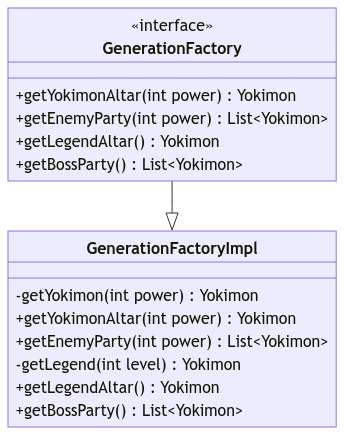
\includegraphics[width=0.55\columnwidth]{images/uml-generator-factory.png}
\caption{Schema UML della \texttt{GenerationFactory} e della sua implementazione}
\label{img:uml-generator-factory}
\end{figure}
\paragraph{Problema} Gli \texttt{Yokimon}, sia quelli ricevuti dagli altari sia quelli usati dagli \texttt{Enemy} in combattimento, vengono generati randomicamente in base a quanto il \texttt{Player} è distante dal centro della mappa.
\paragraph{Soluzione} Per risolvere questa esigenza ho utilizzato il factory method, rispettando i principi DIP, OCP e SRP. 
%
Le altre classi possono creare un \texttt{GenerationFactory} con costruttore vuoto. 
%
I metodi della classe richiedono un intero, fornitogli da un apposito sottomodulo, rendendo la factory funzionante e bilanciata anche in caso di espansione della mappa di gioco. 
%
Questa factory è facilmente espandibile nel caso di future aggiunte, come nuove entità o tipologie diverse di oggetti. 
%
Per creare speciali nemici con party predefinito non è necessario creare nuove classi, estendendo ad esempio enemy: usando metodi come \texttt{getPartyBoss()} si può sopperire abbastanza facilmente a questa esigenza.
\subsubsection{Marilia Merendi}
\subsubsection{Componenti della logica di combattimento}
\begin{figure}[H]
\centering{}
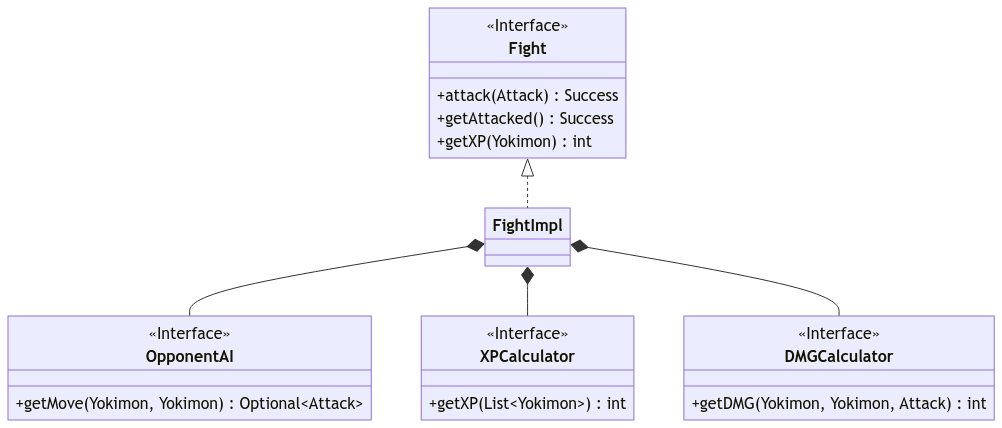
\includegraphics[width=1.0\columnwidth]{images/uml-fight.png}
\caption{Schema UML dell'implementazione delle componenti di \texttt{Fight}}
\label{img:uml-fight}
\end{figure}
\paragraph{Problema} Creare un’implementazione della logica di combattimento che fosse facile da modificare o da estendere.
\paragraph{Soluzione} L’implementazione di Fight fa uso della composition: presenta diversi componenti che determinano l’effettiva logica di combattimento. Essi sono \texttt{OpponentAI}, \texttt{XPCalculator} e \texttt{DMGCalculator}. 
%
Questo scorporamento è impostato per rispettare il Single Responsibility Principle: ognuna di queste componenti è responsabile di un singolo comportamento specifico della logica di gioco. \\
%
Inoltre viene rispettato il Dependency-Inversion Principle: i metodi di \texttt{FightImpl} non dipendono da alcuna specifica implementazione di queste componenti, ma solo dalle loro interfacce.
%
In \Cref{img:uml-opponentai} sono evidenziati i metodi di \texttt{Fight} per i quali la sua implementazione sfrutta le varie componenti. \\
In particolare: 
\begin{itemize}
    \item \texttt{OpponentAI} determina il modo in cui, durante un combattimento, lo \texttt{Yokimon} nemico sceglie quale attacco utilizzare.
    \item \texttt{XPCalculator} determina quanti punti vengono assegnati allo \texttt{Yokimon} del player in caso di vittoria.
    \item \texttt{DMGCalculator} determina l’entità del danno (damage) dato da un attacco, espressa in punti HP da sottrarre e lo Status dell’attacco (ad es. se è un colpo critico).
\end{itemize}
\subsubsection{Implementazione delle componenti di Fight}
\begin{figure}[H]
\centering{}
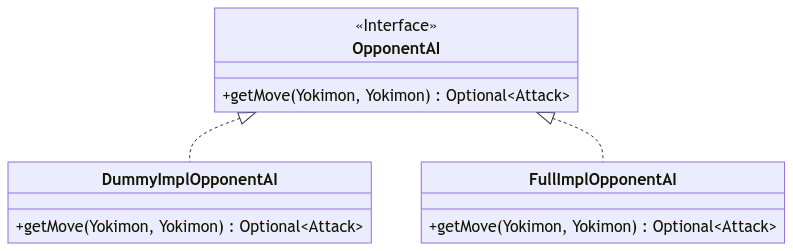
\includegraphics[width=1.0\columnwidth]{images/uml-opponentai.png}
\caption{Schema UML dell'implementazione dell'AI nemica}
\label{img:uml-opponentai}
\end{figure}
\paragraph{Problema} In fase di sviluppo sono stati implementati più algoritmi intercambiabili per le diverse componenti di Fight, realizzati aumentando man mano il grado di complessità.
\paragraph{Soluzione} OpponentAI, XPCalculator e DMGCalculator seguono tutte il pattern Strategy: presentano delle implementazioni che sono una famiglia di algoritmi interscambiabili, dati dalla specializzazione di un’interfaccia di base.
%
\Cref{img:uml-fight}, un esempio relativo a OpponentAI.
\subsubsection{DMG Calculator}
\begin{figure}[H]
\centering{}
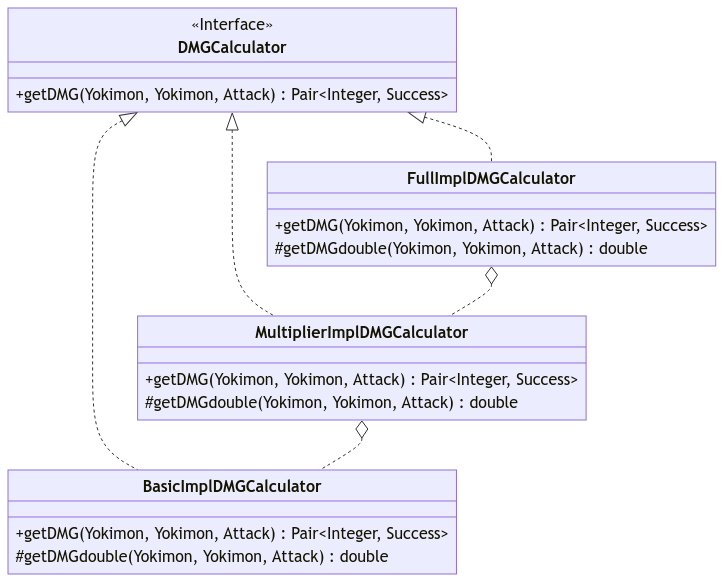
\includegraphics[width=1.0\columnwidth]{images/uml-dmgcalc.png}
\caption{Schema UML delle implementazioni di un \texttt{DMGCalculator}}
\label{img:uml-dmgcalc}
\end{figure}
\paragraph{Problema} Esistono più implementazioni che altro non sono che progressive specializzazioni per calcolare sempre più accuratamente il danno.
%
Serve un modo per evitare ripetizione di codice e rispettare il principio DRY.
\paragraph{Soluzione} Si sfrutta il pattern decorator: la versione più specializzata è un wrapper della versione precedente (in particolare nell’ordine BasicImpl - MultiplierImpl - FullImpl). \\
\footnotesize \\
Nota: Le implementazioni di DMGCalculator dispongono anche di un metodo protected, \textbf{getDMGdouble()}.
%
Serve a ottenere un damage più accurato, prima che il risultato venga troncato ad int per essere utilizzato dall’esterno (da takeDamage(), che richiede un int). Senza questo metodo, il sistema di decoratori darebbe risultati molto più imprecisi, a causa di troncamenti in successione.
\normalsize
\subsubsection{Gestione di eventi}
\begin{figure}[H]
\centering{}
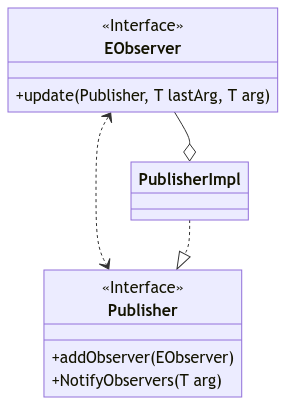
\includegraphics[width=0.4\columnwidth]{images/uml-publisher.png}
\caption{Schema UML della relazione \texttt{Publisher} \texttt{EObserver}}
\label{img:uml-publisher}
\end{figure}
\paragraph{Problema} Serve un sistema per notificare alla View dei cambiamenti a seguito di determinati eventi, alla quale essa poi deve rispondere aggiornando la scene mostrata a schermo. 
%
Questi eventi possono essere di varie tipologie: cambio di posizione del \texttt{Player}, sostituzione di uno \texttt{Yokimon} durante il combattimento, etc.
\paragraph{Soluzione} Seguendo il pattern Observer, è stata impostata un’interfaccia generica \texttt{EObserver}, e un’altra, \texttt{Publisher}, responsabile per la notificazione di eventi.
\subsubsection{Luca Palazzini}
\subsubsection{Tile system}
\begin{figure}[H]
\centering{}
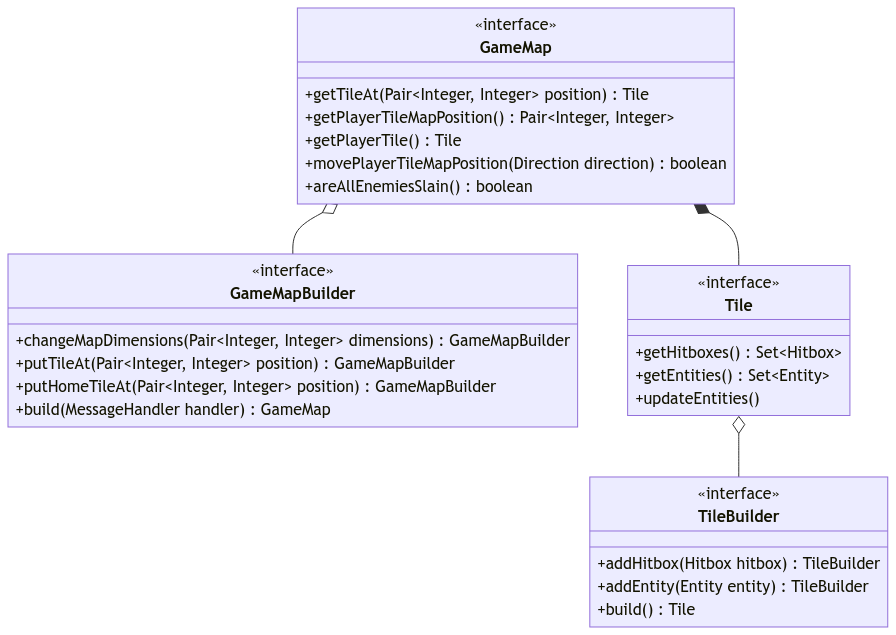
\includegraphics[width=1.0\columnwidth]{images/uml-map.png}
\caption{Schema UML delle relazioni fra la \texttt{GameMap} e le proprie componenti}
\label{img:uml-game-map}
\end{figure}
\paragraph{Problema} Mantenere delle classi per la \texttt{GameMap} ed i tile in un modo estendibile per poter permettere una creazione modulare di \texttt{Tile}.
\paragraph{Soluzione} La creazione della mappa si basa su una collezione di \texttt{Tile}, ovvero schermate di gioco contenute nella \texttt{GameMap}. 
%
Si utilizza il Builder pattern per facilitare la creazione di questi \texttt{Tile}, e permetterne una estensione nel caso si volessero aggiungere funzionalità ad un \texttt{Tile} o averne alcuni con delle specifiche precise.
\subsubsection{Hitbox system}
\begin{figure}[H]
\centering{}
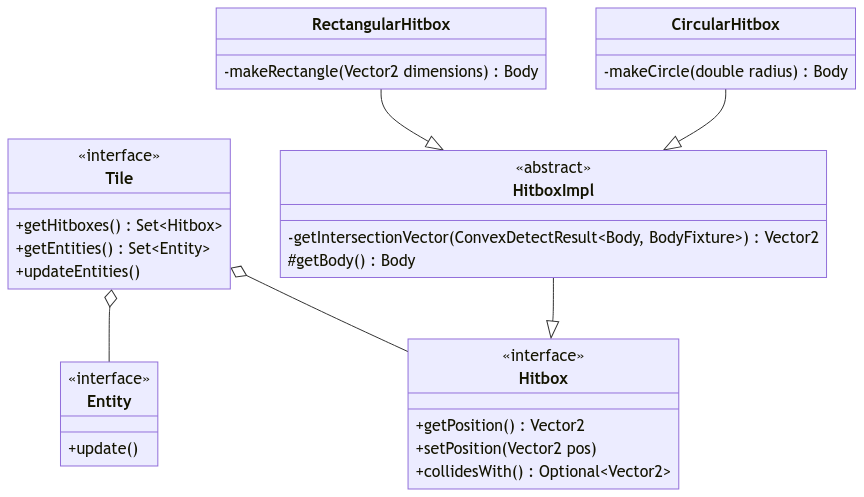
\includegraphics[width=1.0\columnwidth]{images/uml-hitbox.png}
\caption{Schema UML della relazione fra \texttt{Hitbox}, le \texttt{Entity} ed i \texttt{Tile}}
\label{img:uml-hitbox}
\end{figure}
\paragraph{Problema} Fare in modo che il \texttt{Player} non potesse uscire dai confini di un \texttt{Tile}, ed assicurarsi che esso non potesse attraversare ostacoli.
\paragraph{Soluzione} Viene utilizzato il pattern della Dependency Inversion (DI) per assicurarsi di dipendere esclusivamente dalle nostre interfacce, invece della implementazione della libreria da noi utilizzata (dyn4j\footnote{\url{https://dyn4j.org/}}), una libreria che permette di implementare meccaniche di fisica (da noi non utilizzate) e collisioni tra oggetti. 
%
Questi \texttt{Hitbox} vengono posizionati su tutti gli oggetti ed entità di cui vogliamo controllare (ed eventualmente risolvere) collisioni.
\subsubsection{Map generation}
\begin{figure}[H]
\centering{}
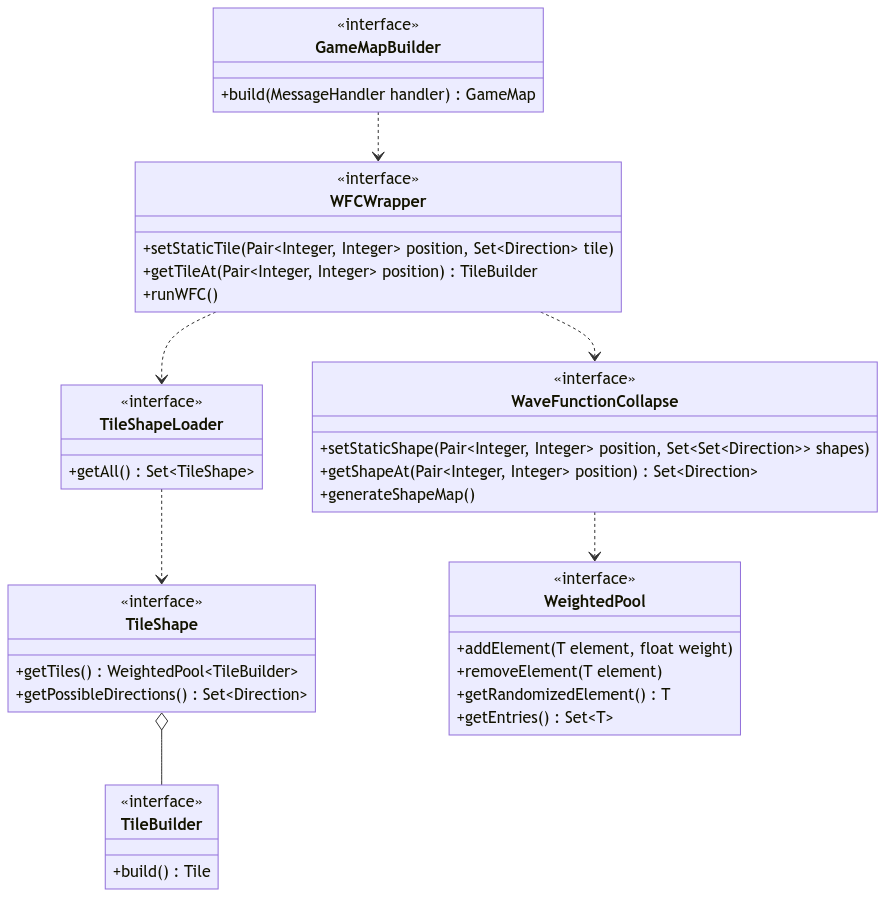
\includegraphics[width=1.0\columnwidth]{images/uml-mapgen.png}
\caption{Schema UML della generazione di una mappa}
\label{img:uml-map-generation}
\end{figure}
\paragraph{Problema} Generare una \texttt{GameMap}, e le \texttt{Entity} contenute in essa, coerente a \texttt{Tile} letti da un file JSON che permette al player di muoversi per tutti i tile connessi della mappa.
\paragraph{Soluzione} La generazione randomica della mappa viene effettuata da un algoritmo chiamato Wave Function Collapse.
%
Inizialmente volevamo utilizzare una libreria per risolvere questo problema ma ne abbiamo trovate solo poco affidabili (ad esempio jwfc\footnote{\url{https://github.com/GameplayJDK/java-wfc}} o l'implementazione di heathensoft\footnote{\url{https://github.com/heathensoft/WaveFunctionCollapse}}).
%
La \texttt{WaveFunctionCollapse} da me implementata gestisce delle “Shapes” definite dalle loro direzioni che permettono all’algoritmo di capire in che direzioni se ne possono connettere altre. 
%
Il \texttt{WFCWrapper} invece ha il compito di tradurre queste shape in \texttt{Tile}, leggendo delle \texttt{TileShape} dal \texttt{TileShapeLoader} per ottenerne uno della rispettiva shape, così facendo si possono aggiungere nuovi \texttt{Tile} specificandoli nel file JSON. 
%
Infine queste \texttt{TileShapeLoader} vengono presi dalla \texttt{GameMapBuilder} che, costruirà i \texttt{Tile} stessi con le proprie \texttt{Entity} ed \texttt{Hitbox}.
\subsubsection{Giovanni Paone}
\subsubsection{Sistema di sottomoduli e event bus}
\begin{figure}[H]
\centering{}
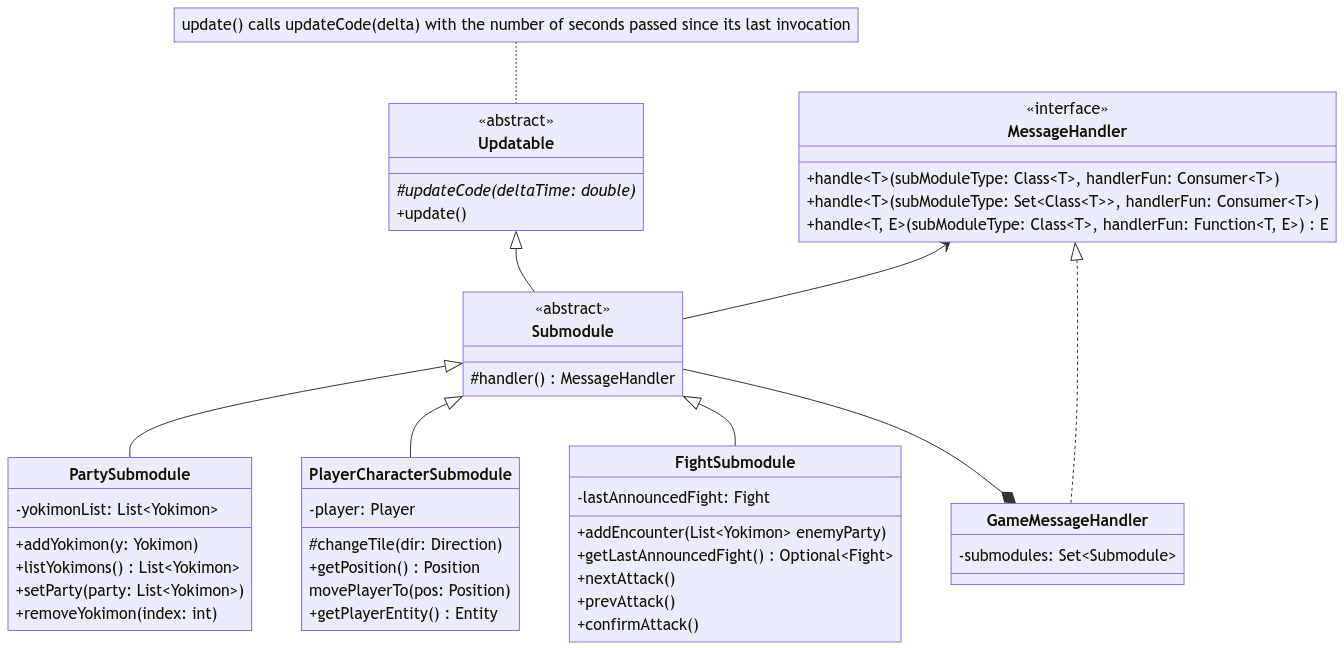
\includegraphics[width=1.0\columnwidth]{images/uml-submodules.png}
\caption{Schema UML dei \texttt{Submodules}}
\label{img:uml-submodules}
\end{figure}
\paragraph{Problema} Non solo abbiamo il problema che le \texttt{Entity} hanno bisogno di un modo per interagire tra di loro (l’altare deve controllare che si sta avvicinando il giocatore, il nemico deve correre verso il giocatore se lo vede e reagire alle collisioni con la mappa o con altre entità), abbiamo anche da considerare che le \texttt{Entity} (oltre ad altri componenti di gioco) avranno la necessità di comunicare anche con parti del gioco (e.g. il nemico deve chiamare l’istanziazione di un combattimento se tocca il player, l’altare deve dare uno yokimon al player una volta che si è avvicinato). 
%
Presupponendo che questi sottomoduli di gioco siano in classi separate (come dovrebbe essere) questo farebbe risalire inoltre la necessità di una comunicazione inter modulo (il sottomodulo che si occupa dei combattimenti deve chiedere il contenuto del party del \texttt{Player} al sottomodulo che se ne occupa).
\paragraph{Soluzione} Per risolvere tutti questi problemi nel modo più generale possibile, ho diviso la funzionalità principale del gioco in sottomoduli (\texttt{Submodule}) e ho creato un bus principale che permette la comunicazione non solo tra \texttt{Submodule} ma anche tra \texttt{Entity} e \texttt{Submodule}, prendendo spunto dal design pattern del Command (anche se usa \texttt{Consumer} piuttosto che una classe command progettata da noi, e non è usata per callback ma viene chiamata appena viene ricevuta dal metodo handle apposito).
\subsubsection{Caricamento da file}
\begin{figure}[H]
\centering{}
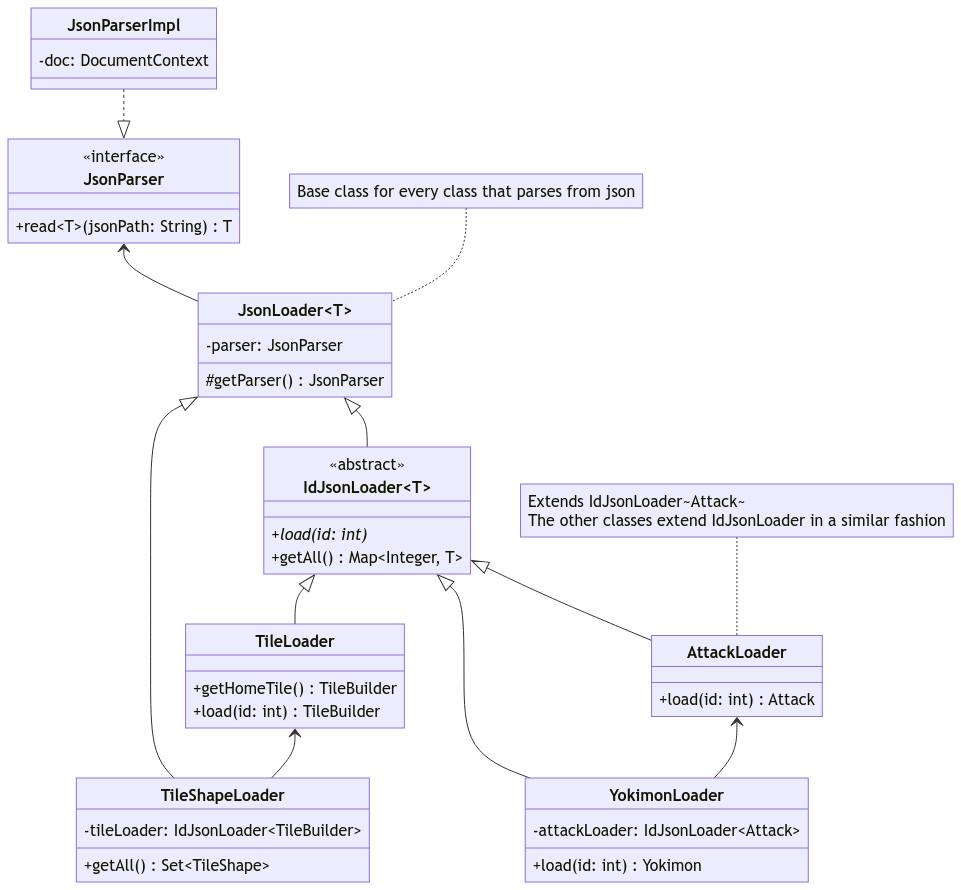
\includegraphics[width=1.0\columnwidth]{images/uml-loaders.png}
\caption{Schema UML dei \texttt{JsonLoader}}
\label{img:uml-loaders}
\end{figure}
\paragraph{Problema} I tipi di \texttt{Yokimon} sono finiti e predeterminati, e la stessa cosa vale per le \texttt{Tile} che usiamo nella generazione della mappa e degli attacchi che contengono gli \texttt{Yokimon}. 
%
Una soluzione sarebbe fare un \texttt{Singleton} che contiene informazioni per istanziare queste classi, ma è una soluzione inelegante e poco scalabile.
\paragraph{Soluzione} Per questo problema ho scelto di tenere le informazioni su \texttt{Tile}, \texttt{Yokimon} e attacchi in file json, per poi utilizzare un parser json dalla libreria di terze parti json-path\footnote{\url{https://github.com/json-path/JsonPath}} (adottando il principio di dependency inversion per garantire la sostituibilità della dipendenza) per istanziare le tre classi e i \texttt{TileShape} necessari per inizializzare la WFC con un’interfaccia comune. 
%
\texttt{IdJsonLoader} e tutte le classi che la estendono adottano il design pattern del factory method.
\chapter{Sviluppo}
\section{Testing automatizzato}
\subsubsection{Entità}
Per il sistema di entità sono state testate le caratteristiche principali di ciascuna delle implementazioni:
\begin{itemize}
    \item Per Enemy, lo stato di Wander e Follow, così come la direzione in cui punta l’enemy durante lo stato di wander.
    \item Per People il fatto che un’entità cambi la direzione dello sguardo tra destra e sinistra in base all’ultimo spostamento effettuato.
    \item Per Player il sistema di movimento.
    \item Per Altar il controllo della corretta acquisizione di Yokimon quando il player è nel suo raggio.
    \item Per effettuare i test per Enemy e Altar, è stato necessario creare una classe a parte per permettere di simulare una mappa incompleta con un certo livello di personalizzazione (AbsTestMessageHandler).
\end{itemize}
\subsubsection{Yokimon}
Per l’implementazione di Yokimon sono stati fatti dei semplici test per controllare che statistiche e attacchi fossero gestiti correttamente durante il level-up e di conseguenza anche il corrispondente guadagno di XP Points con corretto messaggio di ritorno. \\
%
Per la generation factory viene testata la corretta generazione di uno Yokimon, del party nemico e della squadra del Boss (feature presente ma non implementata).
\subsubsection{Fight e le sue componenti}
C’è una classe di test per ogni componente della logica di combattimento: XPCalculator, DMGCalculator e OpponentAI. \\
%
In ciascuna di queste classi di test è presente un metodo per testare ogni implementazione dell’interfaccia. \\
%
Esiste una classe di test anche per Fight, nella quale vengono testati l’istanziazione e le principali funzionalità di Fight, come attack(), getAttacked() e isOver(). \\
%
Tutte le classi di test sono automatizzate e in particolare sfruttano la suite JUnit.
\subsubsection{Game Map e Tiles}
Ci sono classi di test per verificare il calcolo della collisione per gli hitbox, HitboxTest. \\
%
Questi servono per assicurarsi che le entità che collidono non attuino comportamenti inattesi. \\
%
Inoltre ci sono diversi test per controllare le funzionalità della mappa, il movimento del player tra i tile e i loro builder: TileTest, TileBuilderTest, GameMapTest, GameMapBuilderTest. \\
%
Infine vengono anche testate le funzionalità di generazione della mappa e degli algoritmi utilizzati per assicurarsi che i Tile vengano connessi tutti correttamente: WaveFunctionCollapseTest e WFCWrapperTest.
\subsubsection{Utilities}
Classi di test per operazioni fra vettori ed implementazione di una collezione di oggetti generici randomizzata: Vector2Test, WeightedPoolTest. \\
%
Queste classi servono per verificare la corretta implementazione di randomizzazione degli oggetti e, per il vettore, la corretta gestione dei valori che hanno e della loro immutabilità. \\
%
Per la classe Position invece sono stati effettuati dei test per controllare la corretta verifica della posizione nella mappa e inoltre anche la possibilità di determinare se una posizione fosse o meno nel raggio di un’altra.
\subsubsection{File loaders}
Contenuti in io.github.yokigroup.file.loader.*, test automatici che caricando da file json esclusivi al classpath di test verificano il corretto instanziamento da file di attacchi, yokimon e tile.
\section{Note di sviluppo}
\subsubsection{Federico De Leonardis}
Uso di lambda expression nelle chiamate a sottomoduli usate in vari punti. Un paio di esempi sono: \\
Lambda expression in encounter \texttt{Enemy} \\
\textbf{Permalink:} \url{https://github.com/YokiGroup/OOP23-yokimon/blob/50c71f7560acd321b9b7e90acbd569969ba06c56/src/main/java/io/github/yokigroup/world/entity/people/Enemy.java#L154-L157} \\
\\ 
Lambda expression in UpdateCode \texttt{Altar} \\
\textbf{Permalink:} \url{https://github.com/YokiGroup/OOP23-yokimon/blob/50c71f7560acd321b9b7e90acbd569969ba06c56/src/main/java/io/github/yokigroup/world/entity/Altar.java#L80-L90} \\
\\
Uso di stream vari in: \\
collisionCheck \texttt{People} \\
\textbf{Permalink:} \url{https://github.com/YokiGroup/OOP23-yokimon/blob/50c71f7560acd321b9b7e90acbd569969ba06c56/src/main/java/io/github/yokigroup/world/entity/people/People.java#L218-L230} \\
\\
Wander \texttt{Enemy} \\
\textbf{Permalink:} \url{https://github.com/YokiGroup/OOP23-yokimon/blob/50c71f7560acd321b9b7e90acbd569969ba06c56/src/main/java/io/github/yokigroup/world/entity/people/Enemy.java#L119-L124}
\subsubsection{Luca Palazzini}
Utilizzo di generici nella \texttt{WeightedPool}: \\
Permalink: \url{https://github.com/YokiGroup/OOP23-yokimon/blob/64c3de42ddb4b22089bfd5102785fb9b42ed326d/src/main/java/io/github/yokigroup/util/WeightedPool.java#L6-L57} \\
\\
Utilizzo di libreria dynj4 in \texttt{Hitbox}: \\
Permalink: \url{https://github.com/YokiGroup/OOP23-yokimon/blob/50c71f7560acd321b9b7e90acbd569969ba06c56/src/main/java/io/github/yokigroup/world/entity/hitbox/HitboxImpl.java#L44-L74} \\
\\
Utilizzo di stream e lambda in: \\
\texttt{WFCWrapperImpl}: \\
Permalink: \url{https://github.com/YokiGroup/OOP23-yokimon/blob/50c71f7560acd321b9b7e90acbd569969ba06c56/src/main/java/io/github/yokigroup/world/gen/WFCWrapperImpl.java#L45-L55} \\
\\
\texttt{GameMapImpl}: \\
Permalink: \url{https://github.com/YokiGroup/OOP23-yokimon/blob/50c71f7560acd321b9b7e90acbd569969ba06c56/src/main/java/io/github/yokigroup/world/GameMapImpl.java#L44-L53}
\subsubsection{Marilia Merendi}
Progettazione con generici: \\
Nel meccanismo Publisher-Observer. \\
Un esempio: \\
\textbf{Permalink:} \url{https://github.com/YokiGroup/OOP23-yokimon/blob/b217c731c7a877c9898b858ac7a836c2f2006e79/src/main/java/io/github/yokigroup/event/observer/Publisher.java#L7-L20} \\
\\
Utilizzo di Optional: \\
Presenti in vari punti, tra cui: \\
\textbf{Permalink:} \url{https://github.com/YokiGroup/OOP23-yokimon/blob/b217c731c7a877c9898b858ac7a836c2f2006e79/src/main/java/io/github/yokigroup/battle/opponentai/OpponentAI.java#L21}
\subsubsection{Giovanni Paone}
Utilizzo di Optional, progettazione con generici bounded: \\
Presente in vari punti, tra cui: \\
\textbf{Permalink:} \url{https://github.com/YokiGroup/OOP23-yokimon/blob/50c71f7560acd321b9b7e90acbd569969ba06c56/src/main/java/io/github/yokigroup/core/GameMessageHandler.java#L110-L114} \\
\\
Utilizzo di libreria JsonPath: \\
\textbf{Permalink:} \url{https://github.com/YokiGroup/OOP23-yokimon/blob/50c71f7560acd321b9b7e90acbd569969ba06c56/src/main/java/io/github/yokigroup/util/json/JsonParserImpl.java#L27-L36} \\
\\
Uso di Stream: \\
Presente in vari punti, tra cui: \\
\textbf{Permalink:} \url{https://github.com/YokiGroup/OOP23-yokimon/blob/50c71f7560acd321b9b7e90acbd569969ba06c56/src/main/java/io/github/yokigroup/event/submodule/GameStateSubmodule.java#L56-L59} \\
\\
Uso di lambda expressions: \\
Presente in vari punti, tra cui: \\
\textbf{Permalink:} \url{https://github.com/YokiGroup/OOP23-yokimon/blob/50c71f7560acd321b9b7e90acbd569969ba06c56/src/main/java/io/github/yokigroup/event/submodule/abs/GameMapSubmoduleAbs.java#L111-L117} \\
\\
Uso di reflection: \\
\textbf{Permalink:} \url{https://github.com/YokiGroup/OOP23-yokimon/blob/50c71f7560acd321b9b7e90acbd569969ba06c56/src/main/java/io/github/yokigroup/core/GameMessageHandler.java#L62-L70}
\chapter{Commenti finali}
\section{Autovalutazione e lavori futuri}
\subsubsection{Marilia Merendi}
Punti di forza: \\
%
Applicazione dei pattern. \\
%
Particolare attenzione nello sviluppo del Model seguendo il TDD. \\
%
Documentazione esaustiva. \\
%
Più implementazioni per le stesse componenti di Fight (ottimale per TDD, dato che permettono l’implementazione gradualmente più articolata di FightImpl). \\
\\
Punti di debolezza: \\
%
Difficoltà nell’integrare il proprio lavoro con quello degli altri. \\
%
Scarsa comprensione di aspetti avanzati come lambda expressions e streams. \\
%
Scarso contributo alla view e al controller. \\
\\
Il mio ruolo è stato relativo allo sviluppo delle game mechanics necessarie per il combattimento e in parte alla creazione del sistema di Publisher e Observer, che è stato sfruttato in vari punti del programma per la comunicazione tra Model e View.
%
Ho dato un contributo significativo alla relazione.
\subsubsection{De Leonardis Federico}
Punti di forza: \\
%
Applicazione dei Pattern. \\
%
Grande estensibilità della classe astratta entity. \\
%
Praticità della classe Yokimon nel fight-system e nel loader durante il caricamento da file. \\
%
Uso moderato ma abbastanza efficace di stream e lamba nel sistema di entità. \\
%
Parte attiva nell’ideazione delle funzionalità del gioco e dell’organizzazione. \\
\\
Punti di debolezza: \\
%
Mancata conoscenza di aspetti più avanzati delle parti dei compagni con conseguente rallentamento del lavoro. \\
%
Comunicazione non sempre chiara con conseguenti fraintendimenti e cambiamenti di model in corso d’opera. \\
%
Contributo non ottimale al di fuori della mia parte o da quella organizzativa/ideazionale. \\
\subsubsection{Palazzini Luca}
Punti di forza: \\
%
Applicazione di pattern e generici. \\
%
Utilizzo ottimale di stream ed eventuali lambda per migliorare la lettura e qualità del codice. \\
%
Corretta implementazione di classi seguendo il Dependency Inversion Principle, principalmente riguardanti classi di librerie esterne. \\
\\
Punti di debolezza: \\
%
Comunicazione non sempre buona con i compagni di lavoro, rendendo difficile capire e di conseguenza implementare funzionalità necessarie per facilitare il lavoro agli altri. \\
%
Estendibilità del codice scritto non ottimale.
\subsubsection{Giovanni Paone}
Punti di forza: \\
%
Ossessione al dettaglio: Dalla scelta della gerarchia dei package alla struttura dei messaggi di commit mi sono dato l’obiettivo di aiutare il gruppo a mantenere uno standard di qualità nei confronti del dettaglio. \\
\\
Per quanto riguarda portare avanti il progetto, io e i miei colleghi stiamo considerando l’idea.
%
Il concept più inverosimile da raggiungere a cui abbiamo pensato è di introdurre una meccanica di multiplayer, ma richiederebbe un considerevole impegno non solo per implementarlo come l’avevamo ideato ma richiederebbe anche una rifinitura delle meccaniche già presenti in termini di bilanciamento e UX per essere considerato un gioco e non più solamente un progetto tecnico. \\
\\
Punti di debolezza: \\
L’ossessione al dettaglio è un’arma a doppio taglio, specialmente se i tempi non lo permettono. \\
%
Difficoltà a stare concentrato: La difficoltà maggiore che ho riscontrato in questo progetto non è stata l’architettura del gioco in sé, ma la mia concentrazione e il tempo effettivo che trascorrevo a programmare.
%
Nonostante possa sembrare che il volume di codice che abbia prodotto abbia superato di gran lunga le 70 ore, le mie stime mi suggeriscono che le abbia superate ma non di troppo. \\
%
Uno dei miei difetti più grandi è che non riesco a lavorare (anche a cose che mi piacciono) per periodi prolungati di tempo, e lo stress causato dalla pressione della sessione e dal ritardo che ha causato al progetto ha solamente intensificato questo difetto.

\section{Difficoltà incontrate e commenti per i docenti}
\subsubsection{Marilia Merendi}
Premetto che prima di questo corso non avevo alcuna conoscenza del linguaggio Java. \\
%
Forse alcuni aspetti vanno approfonditi maggiormente in aula prima di essere visti in laboratorio, soprattutto aspetti avanzati come lambda e stream wmeritano più tempo. \\
%
Ho riscontrato grosse problematiche col fattore tempo nella prova di laboratorio: dal mio punto di vista, il margine di tempo che si può dedicare al ragionamento o all’errore è davvero risicato e sono riuscita a svolgere in tempo diverse prove solo se avevo un’idea implementativa sin dal principio. \\
%
Ciononostante, il corso mi è sembrato davvero completo, soprattutto per la quantità di tool per la programmazione che vengono presentati e per la forma mentis che permette di sviluppare, rivolta soprattutto al concetto di buona programmazione.
%
\subsubsection{Federico De Leonardis}
La mia esperienza in questo progetto java è stata abbastanza travagliata. 
%
Prima di iniziare a lavorarci avevo delle lacune significative riguardo il linguaggio java. 
%
Non avendo mai affrontato a livello scolastico la programmazione a oggetti e neanche in altri linguaggi mi sono sentito un po’ disorientato nell’affrontare un lavoro di gruppo partendo da zero. 
%
Spesso mi sono ritrovato a chiedere aiuto ai compagni con più esperienza, poiché non sapevo bene da dove cominciare. 
%
Durante  la sessione è stato molto dura conciliare il lavoro su questo progetto con gli altri esami, specialmente se si considerano le mie difficoltà nel programmare velocemente come studente con disturbo specifico dell'apprendimento. 
%
Nonostante le sfide incontrate, ho tratto molto valore da questa esperienza. 
%
Ho imparato molto sia rispetto alla programmazione funzionale sia anche per le best practices da usare per far aderire il mio codice agli standard richiesti. 
%
In realtà come idea è molto stimolante lavorare per produrre qualcosa interamente pensata da noi studenti. 
%
Ho rivalutato il linguaggio java, che è ora il mio preferito. 
%
L’unica pecca è l’aver sottovalutato la portata di questo compito e averlo di conseguenza vissuto con molta pesantezza i giorni precedenti alla consegna.
\subsubsection{Luca Palazzini}
Avendo già programmato in linguaggi orientati ad oggetti prima di questo corso non ho avuto specifiche difficoltà in ambito di programmazione. 
%
Vorrei soltanto aggiungere che la metrica di avere un “target” di ore da raggiungere non sia un modo corretto per limitare il tempo speso sul progetto: ad esempio uno studente che ha passato diversi anni a programmare ha le capacità di fare molto in 70 ore rispetto ad uno studente che ha iniziato l’anno prima.
\appendix
\chapter{Guida utente}
\textbf{Comandi per il movimento sulla mappa} \\
\textbf{W key}: Muovi verso l'alto \\
\textbf{A key}: Muovi verso sinistra \\
\textbf{S key}: Muovi verso il basso \\
\textbf{D key}: Muovi verso destra \\
--------------------------------------------------- \\
\textbf{Comandi per la selezione} \\
\textbf{A key}: Opzione precedente \\
\textbf{S key}: Opzione successiva \\
\textbf{Enter key}: Conferma \\ \\
\textbf{Tabelle dei contenuti di gioco} \\
\tiny
\begin{tabular}{ |c|c|c| } 
     \hline
     \textbf{Attack} & \textbf{Color} & \textbf{Power} \\ 
     \hline
     \hline
     Shadow Sneak & Black & 50 \\ 
     \hline
     Bite & Black & 60 \\ 
     \hline
     Web & Black & 85 \\ 
     \hline
     Shadow Ball & Black & 90 \\ 
     \hline
     Soul Attack & Black & 100 \\ 
     \hline
     Mock & White & 0 \\ 
     \hline
     Slap & White & 40 \\ 
     \hline
     Scratch & White & 40 \\ 
     \hline
     Tail Swipe & White & 60 \\ 
     \hline
     Extreme Speed & White & 80 \\ 
     \hline
     Nine Tail Smash & White & 140 \\ 
     \hline
     Celestial Gun & White & 175 \\ 
     \hline
     Cut attributes & White & 500 \\ 
     \hline
     Revenge & Red & 60 \\ 
     \hline
     Strong Punch & Red & 80 \\ 
     \hline
     Katana Slash & Red & 90 \\ 
     \hline
     Flame Throw & Red & 95 \\ 
     \hline
     Tsunami & Red & 100 \\ 
     \hline
     Dragon Rage & Red & 120 \\ 
     \hline
     Confusion & Purple & 50 \\ 
     \hline
     Whirlpool & Purple & 60 \\ 
     \hline
     Curse & Purple & 70 \\ 
     \hline
     Psychic & Purple & 90 \\ 
     \hline
     Dream Eater & Purple & 110 \\ 
     \hline
\end{tabular}
\begin{tabular}{ |c|c|c|c|c|c|c| } 
     \hline
     \textbf{Yokimon} & \textbf{Color} & \textbf{Growth Rate} & \textbf{ATK} & \textbf{DEF} & \textbf{HP} & \textbf{SPD} \\ 
     \hline
     \hline
     Yosuzume & Black & Fast1 & 75 & 70 & 70 & 120 \\ 
     \hline
     Yatagarasu & Black & Fast & 85 & 60 & 70 & 120 \\ 
     \hline
     Tsuchigumo & Black & Medium & 90 & 110 & 50 & 60 \\ 
     \hline
     Akugyo & Black & Fast & 85 & 80 & 85 & 65 \\ 
     \hline
     Sazae-oni & White & Medium & 20 & 300 & 50 & 20 \\ 
     \hline
     KAPPA & White & Medium & 65 & 150 & 75 & 75 \\ 
     \hline
     Tanuki & White & Fast & 75 & 100 & 100 & 70 \\ 
     \hline
     Inugami & White & Slow & 100 & 100 & 100 & 100 \\ 
     \hline
     SonWukong & White & Slow & 120 & 120 & 120 & 120 \\ 
     \hline
     Oni & Red & Medium & 80 & 100 & 90 & 40 \\ 
     \hline
     Tengu & Red & Medium & 95 & 70 & 95 & 110 \\ 
     \hline
     Wani & Red & Slow & 120 & 65 & 120 & 80 \\ 
     \hline
     Baku & Purple & Medium & 75 & 100 & 95 & 75 \\ 
     \hline
     Nekomata & Purple & Medium & 90 & 70 & 110 & 75 \\ 
     \hline
     Kitsune & Purple & Medium & 90 & 90 & 90 & 90 \\ 
     \hline
     Woman & Purple & Fast & 110 & 50 & 50 & 110 \\ 
     \hline
\end{tabular}
\normalsize
\chapter{Esercitazioni di laboratorio}
\subsection{federico.deleonardis@studio.unibo.it}
\subsection{luca.palazzini3@studio.unibo.it}
\subsection{marilia.merendi@studio.unibo.it}
\subsection{giovanni.paone@studio.unibo.it}
\bibliographystyle{alpha}
\bibliography{13-template}
\end{document}